%!TEX root = ../../dissertation.tex
%%%%%%%%%%%%%%%%%%%%%%%%%%%%%%%%%%%%%%%%%%%%%%%%%%%%%%%%%%%%%%%%%%%%%%%%%%%%%%%%
\subsection{Proposal for Cross-Layer Enhancements}
\label{c5:crosslayerhinting}


Wired Internet access has a very narrow choice of protocols on the \gls{ISO}/\gls{OSI} Layers 1 and 2. The typical use-case consists of a \gls{LAN} using Ethernet which is then tunneled through or translated into one of several access technologies, e.g., \gls{DSL}, \gls{DOCSIS}, or \gls{PON}. Applications often make assumptions that rely on the presence of these protocols and their specific characteristics.

However, Internet access today is similarly often achieved using mobile cellular networks. The latest standardized iteration of these is \gls{LTE} and the accompanying \gls{EPS} core network infrastructure \cite{olsson2009sae}. This is the first evolution of standards that completely removes the classical circuit switched domain making room for more radio frequency bandwidth to be used with the all-\gls{IP} services achieving shared transmission capacities --- comparable to today's 802.11n WiFi --- albeit on much larger cell sizes of \SI{1}{\kilo\meter} to \SI{3}{\kilo\meter}. The \gls{EPS} network acts as an intermediary between the radio access stations and the Internet enabling strong traffic control mechanisms as well as mobility anchored at the \gls{SGW}. Traffic is routed through the core by using tunneling over the \gls{SGW} and \gls{PGW} based on the traffic bearer concept defined either in the \gls{gtp} or the \gls{PMIPv6} protocols. For every mobile device connected to the network there is one default and up to ten dedicated bearers carrying traffic filtered by pre-set \gls{QoS} parameters. Control is enforced through a logically separate network control plane, that is also used to setup and tear down these bearers. Figure fig:ltestack displays the disparity between the Internet's protocol stack and that of an \gls{LTE} network encapsulating all user traffic in additional protocol layers by the tunneling process.

Research work is ongoing how to best work with this complex network setup. It is expected, that with the rise of mobile access the core network comes under heavy traffic pressure with negative affects on the \gls{QoS} of best-effort traffic. Endeavors are required to study the loaded network's behavior. Also very little work has gone into exploring the control plane characteristics of these networks, including their performance. A novel approach could also be, to make mobile device applications, e.g. video streaming players, aware of the core networks capabilities and allow the request of tunnels tailored to their specific \gls{QoS} requirements resulting in a possible increase of perceived quality.

% influence of signaling plane and core network elements - scaling

The protocols used for the radio transmissions behave very differently when compared to Ethernet and assumptions made by higher layers may not hold any more. This can apply to, e.g., reliability, frame sizing and fragmenting, and latency amounting to undesired effects on higher-layer traffic. For example, loss in \gls{GSM} and \gls{UMTS} networks is often caught transparently on layer 2 and a retransmission is conducted. However, in the time the retransmission takes the transport layer may have already run into a timeout and re-requested the missing segment on its own, resulting in additional delay and a waste of bandwidth. This is especially detrimental for time-critical applications like video streaming, possibly resulting in buffer underruns and degraded quality. Transport and application layer mechanisms need to be able to understand this and cope with the effects. E.g., \gls{TCP} retransmissions and congestion control could be adjusted in the course of understanding this.

Furthermore, traffic could be avoided during cell handover occurrences. This would require cross-layer cooperation and an awareness of the application when an handover is supposed to occur. The application then could schedule its traffic accordingly. Traffic falling into a handover is subject to especially high latency and loss because the mobile network acts as a mobility anchor which needs to internally reroute incoming traffic to the mobile device's new position. \gls{HTTP} traffic is especially suited to this scheduling behavior because of its statelessness and consistence of small objects that can be requested and transferred independently.

\begin{figure}[htb]
	\centering
	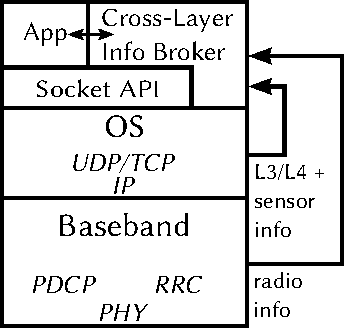
\includegraphics{images/cross-layer-model.pdf}
	\caption{Model and architecture of the proposed cross-layer information exchange.}
\label{c5:fig:crosslayer-model}
\end{figure}


\subsubsection{Related Work}

 ECN~\cite{rfc3168} (one of the earlier notions of cross-layer interactions; disabled by default almost everywhere)

\begin{itemize}
	\item Cross-layer design optimizations in wireless protocol stacks \cite{Raisinghani2004720}
	\item ECLAIR: An efficient cross layer architecture for wireless protocol stacks \cite{raisinghani2004eclair}
	\item Still no implementation of ECLAIR: ``Cross-layer feedback architecture for mobile device protocol stacks'' \cite{1580937}
	\item 802.21
	\item A multi-layer mobility management architecture using cross-layer signalling interactions\cite{wang2003multi}
	\item 
		\begin{itemize}
			\item \gls{DLEP} \cite{ietf2013dlepdraft}
			\item running on routers for communication between routers and attached interfaces (wireless!)
			\item interface/modem informs router about link characteristics
			\item router acts upon this information
			\item specific set of required and optional signals (message types / reason for messaging) and data items (information)
			\item bandwidth, latency, connection status (loss)
			\item information about specific neighbors
			\item \gls{UDP}-based, discovery mechanism via multicast, session-based
			\item requires/relies on lower layer auth/crypt
			\item no data items specific for cell-type mobile nets and mobility
			\item best suited for routers with external modems/interfaces (outside antennas)
		\end{itemize}
	\item Seamless Mobility in Heterogeneous Wireless Networks \cite{zarai2010seamless}
	\item Radio resource management in emerging heterogeneous wireless networks \cite{Piamrat20111066}
	\item Improved community network node design using a DLEP based radio-to-router interface \cite{6379143}
	\item Cross-layer signalling for next-generation wireless systems \cite{1200522}
	\item Cross-layer design for wireless networks \cite{1235598}
	\item A cautionary perspective on cross-layer design \cite{1404568}
	\item User-centric mobility management for multimedia content access \cite{bolla2011usercentric}
	\item Socketless \gls{TCP} --- an end to end handover solution \cite{1635680}
	\item SATSIX cross-layer architecture \cite{4656786}
	\item mostly routing protocol optimization oriented ``A cross layer based QoS model for wireless and mobile ad hoc networks'' \cite{krishna2007cross}
	\item SmoothIT mechanisms; lower layer elements provide information to higher layers, overlays\footnote{\url{http://www.smoothit.org}}  \cite{oechsner2009pushing}
	\item ``Mobility Awareness'' \cite{hummel2010mobilitaet} PMLAR (Predictive mobility and location-aware routing protocol in mobile ad hoc networks)
	\item Automatic Multi-interface Management Through Profile Handling \cite{Bonnin:2009:AMM:1503496.1503498}
	\item A ubiquitous mobile communication architecture for next-generation heterogeneous wireless systems \cite{1452832} (supposed to propose a function that determines the best handover initiation time in order to avoid early or late initiations)
	\item Optimized video streaming over 802.11 by cross-layer signaling \cite{1580941}
	\item LCP Link Control Protocol, PPP extension RFCs \cite{rfc1570,rfc1661}
 	\item Modem Link Properties Advertisement Protocol\footnote{\url{https://tools.ietf.org/html/draft-ivancic-mobopts-modemlpa-01}}
	\item IEEE 802.21 cooperative handovers, but with required network support
	\item LISP and other mobility approaches \cite{rfc6830}
	\item Radio Resource Management RRM
		\begin{itemize}
			\item resource monitoring, decision making, decision enforcement
			\item choose available wireless interfaces  best suited for a specific task
			\item rudimentary implementations in mobile OSs
		\end{itemize}
\end{itemize}




%%
\subsubsection{Cross-Layer Mobility Hinting}

Today's mobile networks are all of a cellular design. A device that moves from one cell to the other has to perform a so-called handover. During this process the device is deregistered in one cell and registered in the new one. All network traffic currently in flight has to be rerouted or relayed to the device's new location. 
Although seemingly transparent to the device's application, adverse side effects can occur during a handover, including an increase and variability of latency. 

Mobility support today always means network assisted mobility. Typically, the network decides the best possible mobility strategy from its point of view and provides infrastructure to support seamless handovers in the form of mobility anchor nodes. However, the device is actually in a very unique position, as it knows a great deal more about its traffic mix, its currently running applications and its user than the network ever could and should.
Unfortunately, most of this information remains unused, as today's network infrastructures and lower layer protocol stacks provide only very slim changes to exert control over decisions regarding the device.

Nonetheless, a lot could still be done when providing the device's operating system and application ecosystem with a simple bidirectional pathway for vertical information and control flow across network protocol layers and to other low-level systems. This work aims to do just that by providing a generic interface and exchange protocol for any kind of information relevant to an application's decision making process. With this meaningful actions and reactions of individual layers can be defined and tested. Possible use cases are provided in the next section.

Still, one has also to keep in mind, that layering and encapsulation is there for a reason and violating this is a rather risky undertaking. However, we do not think that our approach actually violates these basic principles and only extends on the ways one can communicate and interact with all individual layers without changing anything in them.


	% - Research objectives
	% 	- Bidirectional vertical information and control flow on the performance of the individual layers
	% 		- Definition of generic interfaces
	% 		- Definition of a protocol (including information types, etc.)
	% 	- Definition of meaningful actions/reactions on the individual layers (e.g. adaptation of real-time communication data sources or changes in resource allocation)

		

\subsubsection{Scenario Use Cases}

\begin{itemize}
	\item Video/Voice calls that notify the other party, that interruptions are expected to occur.

	\item Using current location data and movement patterns/predictions to improve cell selections and initiate horizontal and vertical handovers to a time suitable for the device and running applications.

	\begin{figure}[htb]
	        \centering
	        \begin{subfigure}[b]{0.90\textwidth}
	            \centering
				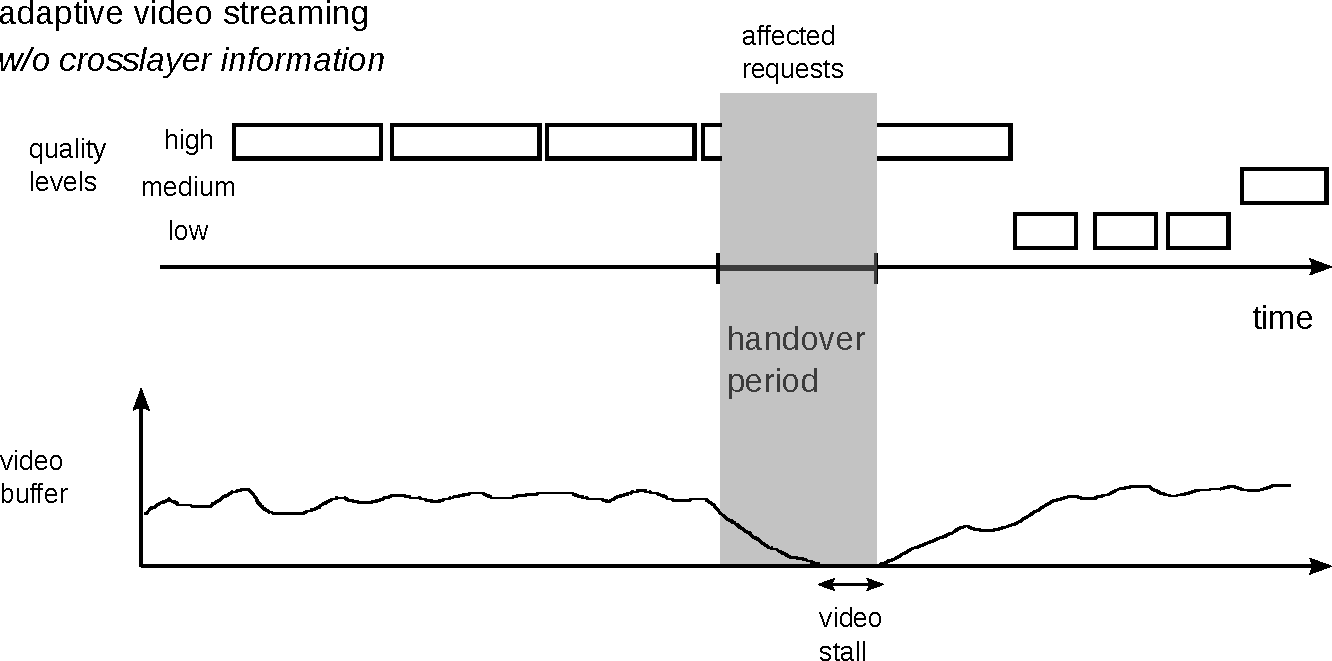
\includegraphics[width=\textwidth]{images/adaptive-streaming-no-cl.pdf}
				\caption{Stalling occurs without handover hinting.}
				\label{c5:fig:streaming-hinting-no-cl}
	        \end{subfigure}%

	        \begin{subfigure}[b]{0.90\textwidth}
				\centering
				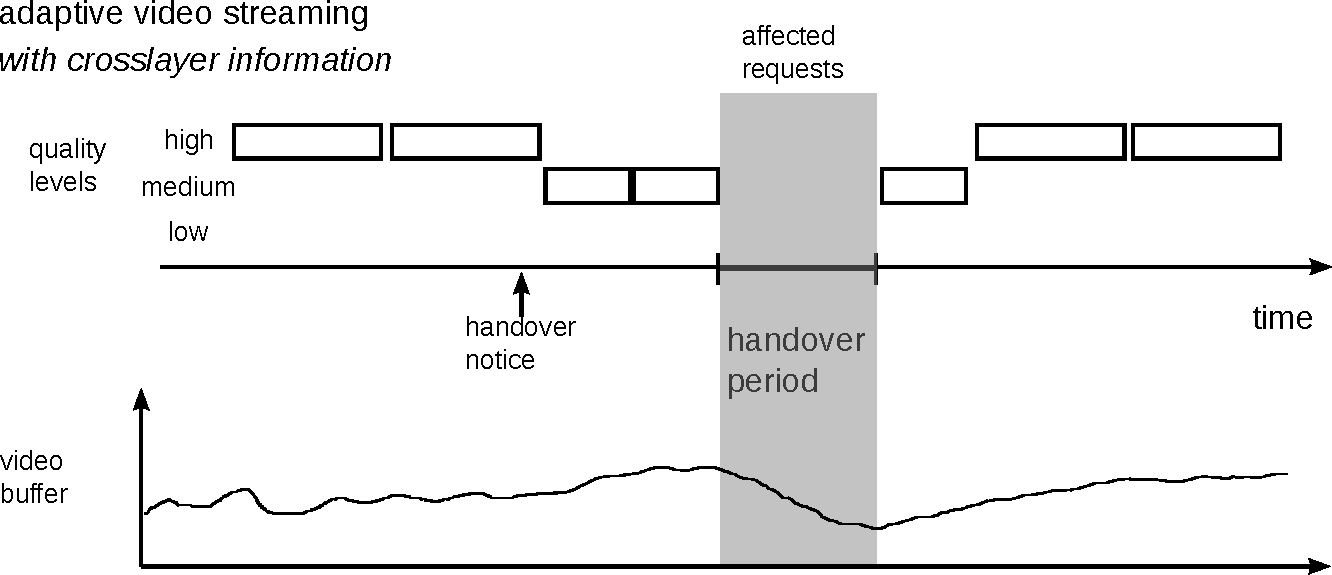
\includegraphics[width=\textwidth]{images/adaptive-streaming-cl.pdf}
				\caption{Stalling can be prevented by hinting and proactively filling the playback buffer.}
				\label{c5:fig:streaming-hinting-cl}
			   \end{subfigure}%
	 \caption{Mockup of handover prediction and hinting for adaptive streaming and thus avoiding playback stalls.}
	\label{c5:fig:streaming-hinting}
	\end{figure}

	\item An adaptive streaming video application increases its video buffer when a shortly upcoming handover is announced to survive the service outage. This can be achieved by an increased rate of segment retrieval and a reduction in segment quality. The goal is to avoid any possible playback stalls due to the handover. Figure~\ref{c5:fig:streaming-hinting} demonstrates this circumstance.

	\begin{figure}[htb]
	        \centering
	        \begin{subfigure}[b]{0.90\textwidth}
	            \centering
				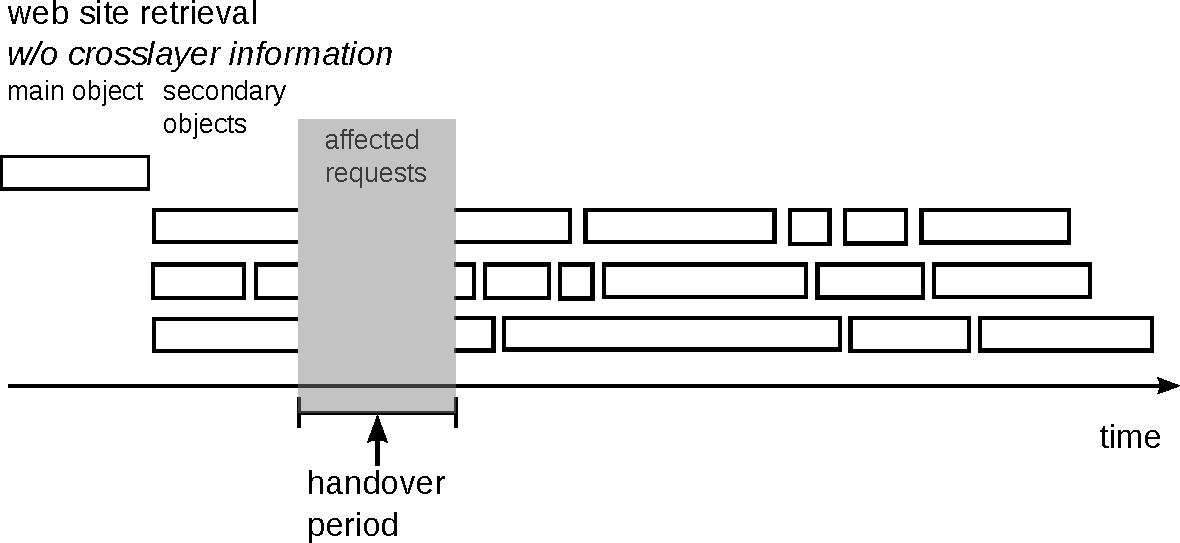
\includegraphics[width=\textwidth]{images/http-reorder-no-cl.pdf}
				\caption{The handover will block currently active object transmissions, page display will be delayed.}
				\label{c5:fig:http-reorder-no-cl}
	        \end{subfigure}%

	        \begin{subfigure}[b]{0.90\textwidth}
				\centering
				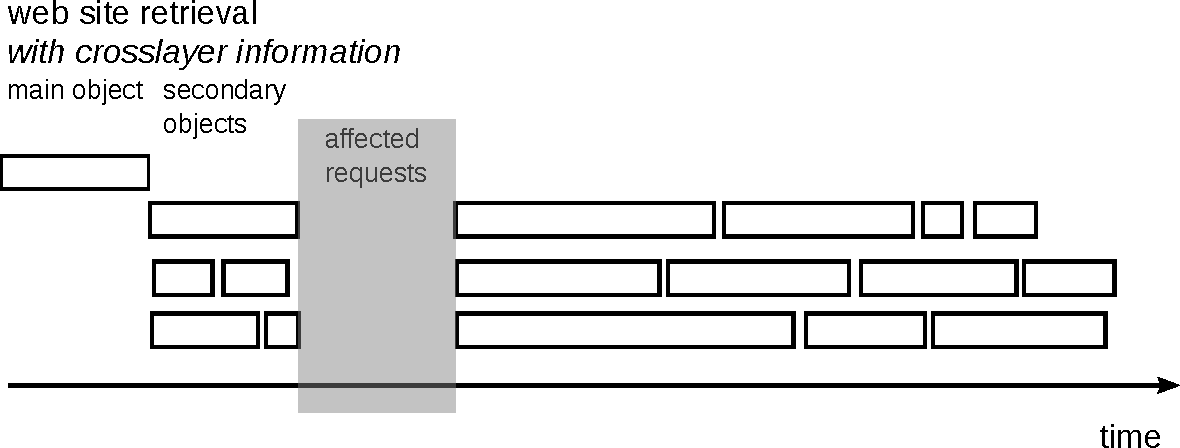
\includegraphics[width=\textwidth]{images/http-reorder-cl.pdf}
				\caption{The browser reorders the objects to be retrieved and avoids any transmissions during the indicated handover period.}
				\label{c5:fig:http-reorder-cl}
			   \end{subfigure}%
	 \caption{Mock-up of \gls{HTTP} reordering with handover awareness.}
	\label{c5:fig:http-reorder}
	\end{figure}

	\item Enable applications to adapt themselves to the conditions currently experienced by the networking stack and its sensors. For example, a Web browser could reorder its Website object requests to avoid sending any requests during handover periods and experience additional delay as seen in Figure~\ref{c5:fig:http-reorder}.

	\item A cross-layer enabled device can also offer a wide range of policy choices to its applications or even directly to the user. An example rule could be: ``Do not handover to a stationary WiFi from 3G when moving faster than 50km/h, only to in-vehicle WiFi.'' or ``Avoid any vertical handover, which would interrupt my service for a long time, while this VoIP call is running.''

\end{itemize}

\subsubsection{Technical Implementation}

The Implementation:
\begin{itemize}
	\item Userspace daemon that collects information from kernelspace protocol implementations and sensors and provides them to all applications.
	\item shared bus control/information system, instead of explicit comm; signaling only to interested parties
	\item provide common interface also to all available sensors and layer 1 and 2 network information and control (similar to Android)
	\item IPC message bus, possibly D-Bus\footnote{\url{http://www.freedesktop.org/wiki/Software/dbus/}} based
	\item Could extend NetworkManager\footnote{\url{https://wiki.gnome.org/Projects/NetworkManager}}, some functionality is already provided there

\end{itemize}

The process:
\begin{itemize}
\item Tell Transport/Application the expected time till handover / time of uninterrupted service
\item Tell Transport/App expected connection parameters (latency, BW, ...)
\item Application selects \gls{DASH} stream appropriate to parameters
\item Application reorders \gls{HTTP} GETs so that large GETs are not interrupted
\item Application stops transfers when handover is about to occur
\item Layer 1/2 gives a list of possible handovers to Application
\item Application selects (better: suggests) handover which fits best and reorders accordingly
\end{itemize}


\subsubsection{Example Benefits}

Put into relation:

\begin{itemize}
	\item frequency of handovers / distance/density of radio towers vs scenario traveling speed
	\item bit-length of streaming segments, typical transmission speed
	\item typical video length and number of segments
	\item derive number of interruptions in segments due to handovers
	\item estimate typical handover/mobility duration and service interruption time per event
	\item sum it up and compare to crosslayer information or even application layer handover decision

\end{itemize}


\subsubsection{Planned Work and Methodology}

\begin{itemize}
	\item investigate how much information is exposed and what can already be done
	\item Analysis of data traces and realistic simulations in order to capture in detail the unwanted phenomena
	\item Verify the suitability of the State-of-the-Art algorithms and protocols which address this problem
\end{itemize}


